Los drones Crazyflie se han utilizado en líneas de investigación relacionadas con sistemas de control y robótica de enjambre debido a su extensa documentación y versatilidad para desarrollo de algoritmos. Para poder realizar un control eficiente de múltiples agentes, es necesario implementar un sistema que sea capaz de obtener y procesar información acerca del comportamiento de los agentes en tiempo real.
\subsubsection*{Crazyflie 2.1}

Los drones a trabajar durante esta línea de investigación son los Crazyflies 2.1, los cuales son cuadricópteros de tamaño pequeño, que pueden ser controlados mediante un sistema de control de enjambre llamado Crazyswarm, el cual es utilizado mediante ROS en Ubuntu. 

Anteriormente, se trabajó con estos drones en una línea de investigación pero no en forma de enjambre, sino con un drone únicamente. Se desarrollaron herramientas para el uso individual de estos drones. En primer lugar, se comprobó la compatibilidad de comunicación entre un drone y Python para el análisis de datos, estos se guardan en bruto y se recomendó graficarlos posteriormente mediante Matlab. Se desarrolló una interfaz gráfica para prácticas de laboratorio, en la cual, se pudo observar el comportamiento del drone ante las propiedades de control determinadas, en este caso, un controlador PID y sus respectivas constantes. Cabe destacar que para poder hacer esta herramienta fue necesario plantear un modelo matemático a través del identificador de sistemas de Matlab. Como resultado de estas herramientas, se llegaron a planificar 2 prácticas de laboratorio para los cursos de Sistemas de Control. \cite{Sanabria2022_tesis}

\subsubsection*{Ecosistema Robotat}

El objetivo principal es utilizar este enjambre de drones en el ecosistema Robotat, el cual es un entorno tecnológico ubicado en el laboratorio de Robótica CIT-116 de la Universidad del Valle de Guatemala. \cite{Camilo2022_tesis}Se implementó un sistema de captura de movimiento mediante un set de 6 cámaras de la marca OptiTrack, las cuales están conectadas a un switch que se comunica con una computadora mediante UDP, también fue implementado un protocolo MQTT para establecer una comunicación Wi-Fi. La información recopilada es procesada mediante un algoritmo de Python y luego es enviada a un router que genera una red Wi-Fi local a la cual es posible conectar diferentes dispositivos y obtener datos como posiciones lineales y angulares. Las cámaras están colocadas de tal forma que rodean una tarima hecha de concreto y acero, como se muestra en la Figura \ref{fig:Robotat}. 

\begin{figure}[t]
    \centering
    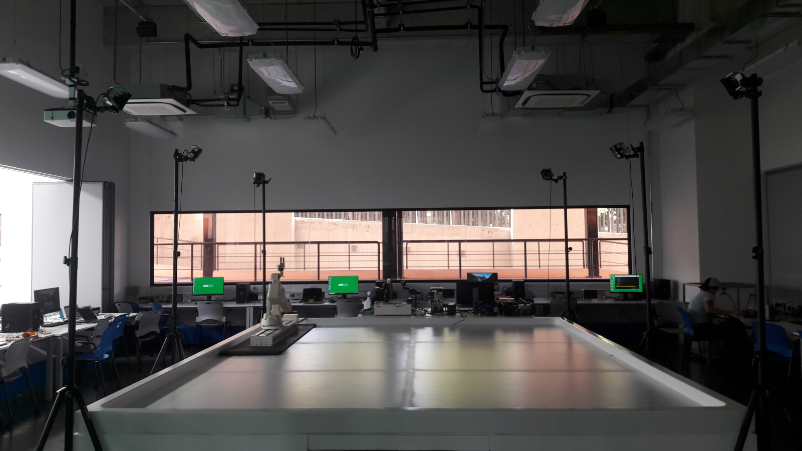
\includegraphics[width=0.5\textwidth]{figuras/Robotat.png}
    \caption{Ecosistema Robotat.}
    \cite{Camilo2022_tesis}
    \label{fig:Robotat}
\end{figure}

\subsubsection{Crazyswarm y ROS2}

ROS es un sistema operativo para sistemas robóticos, el cual provee funciones especiales que facilitan el análisis y control en proyectos de robótica. Este suele trabajarse en sistemas basados en Linux como Ubuntu. A través de ROS2 puede trabajarse Crazyswarm, el cual es un sistema para controlar enjambres de drones Crazyflie 2.1, además se cuenta con un cliente llamado Bitcraze, el cual está basado en Python y permite la comunicación entre el servidor y los drones mediante telecomunicación por radiofrecuencia, este es un sistema independiente de ROS. El entorno Crazyswarm está siendo reemplazado por la versión 2, a la cual se le han estado trabajando mejoras. 

El posicionamiento de los drones se ha realizado de múltiples maneras en distintas líneas de investigación, entre la documentación oficial de Crazyswarm puede encontrarse información sobre pruebas realizadas en sistemas de captura de movimiento, tales como OptiTrack. Para poder realizar experimentos con OptiTrack es necesario implementar un módulo con marcadores reflectivos y este debe estar diseñado a la medida para que el drone pueda ser detectado por las cámaras. Otros métodos utilizados para el posicionamiento de drones es mediante un dispositivo Kinect de la marca Microsoft, utilizado en consolas Xbox. \cite{Crazyswarm}

